% 图 44.1 —— 由 `checks/emit_hand.py` 自动拼出（probe 精测 + prims2 图元分解）
%%
% ⚠ 这是**稿子不是成品**：跑 `checks/checkhand.py 44.1` 看指标 + 看叠合图。
%%
%% ⚠ 待核：
%   · 本图 probe 报出阴影族 1 个 —— **本脚本不生成阴影**（要照原书手写）；prims2 的 strokes 里可能含阴影线，核对时留意别画重
%   · 可疑字形 1 项（空心圈 ⊙ 常被认成字母 o）—— 见文件末
%%
\documentclass[12pt]{standalone}
\usepackage{fontspec}
\setsansfont{Arial}
\newfontfamily\mfallback{DejaVu Sans}
\usepackage{tikz}
\begin{document}
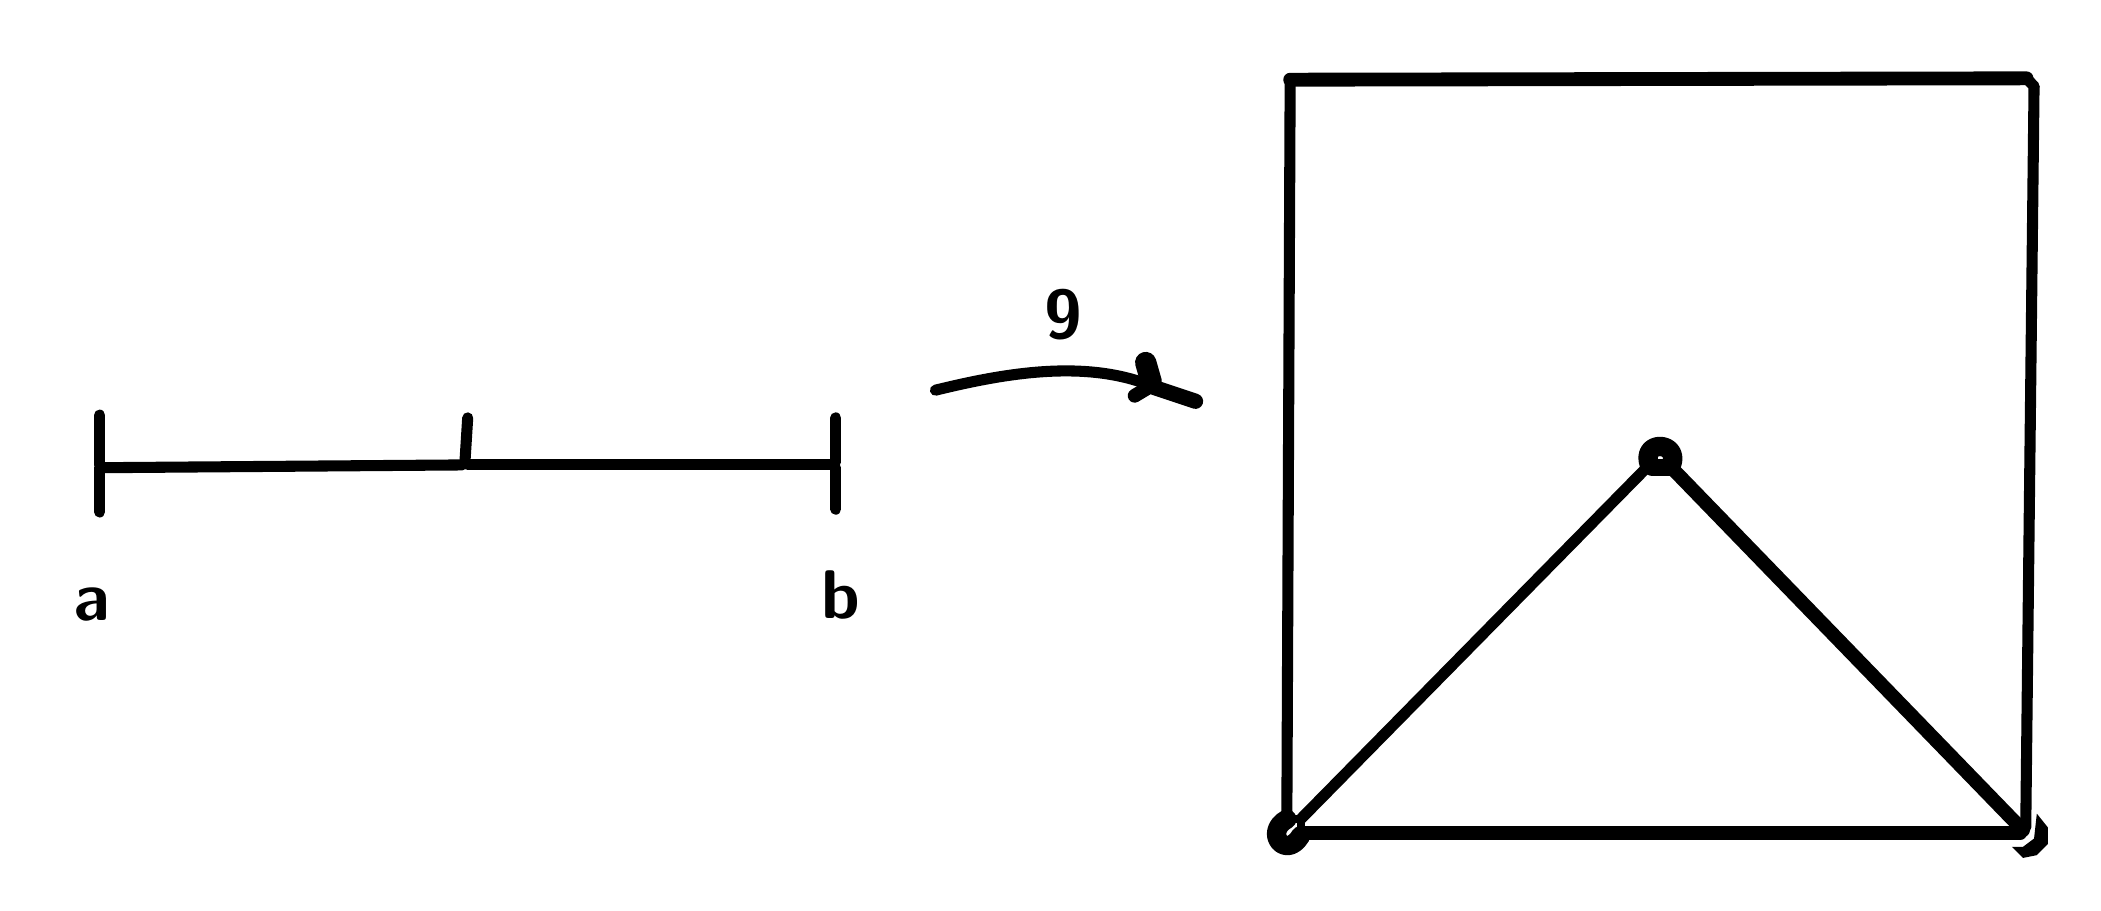
\begin{tikzpicture}[x=1pt, y=-1pt, line width=5.5pt, line cap=round, line join=round]

  %% ════ 填充区（prims2 的 fills）════
  \fill (726.0,284.0) -- (725.0,293.0) -- (721.0,296.0) -- (717.0,296.0) -- (721.0,300.0) -- (726.0,299.0) -- (730.0,295.0) -- (730.0,289.0) -- cycle;

  %% ════ 直线段（prims2 的 strokes）════
  \draw[line width=5.5pt] (422.0,135.0) -- (407.0,130.0);
  \draw[line width=5.0pt] (405.0,130.0) -- (400.0,133.0);
  \draw[line width=4.0pt] (460.0,286.0) -- (585.0,159.0);
  \draw[line width=4.0pt] (26.0,159.0) -- (26.0,175.0);
  \draw[line width=4.0pt] (455.0,285.0) -- (456.2,18.8);
  \draw[line width=5.0pt] (456.2,18.8) -- (722.3,18.3);
  \draw[line width=4.0pt] (722.3,18.3) -- (725.0,21.2);
  \draw[line width=4.0pt] (725.0,21.2) -- (722.0,289.0);
  \draw[line width=3.0pt] (460.0,290.0) -- (460.0,287.0);
  \draw[line width=6.0pt] (587.0,159.0) -- (593.0,159.0);
  \draw[line width=3.0pt] (459.0,286.0) -- (456.0,286.0);
  \draw[line width=7.7pt] (404.0,121.0) -- (406.0,128.0);
  \draw[line width=5.0pt] (461.0,291.0) -- (720.0,291.0);
  \draw[line width=4.0pt] (159.0,141.0) -- (158.0,157.0);
  \draw[line width=4.0pt] (26.0,158.0) -- (26.0,140.0);
  \draw[line width=4.0pt] (157.0,158.0) -- (27.0,159.0);
  \draw[line width=5.0pt] (721.0,290.0) -- (594.0,159.0);
  \draw[line width=4.0pt] (292.0,157.0) -- (292.0,141.0);
  \draw[line width=4.0pt] (291.0,158.0) -- (159.0,158.0);
  \draw[line width=4.0pt] (292.0,159.0) -- (292.0,174.0);

  %% ════ 曲线（prims2 的 curves —— 三段式，坐标同为 (y,x)）════
  \draw[line width=7.0pt] (460.0,292.0) .. controls (454.7,300.9) and (446.4,290.8) .. (455.0,286.0);
  \draw[line width=7.0pt] (594.0,158.0) .. controls (597.1,149.3) and (582.7,148.9) .. (586.0,158.0);
  \draw[line width=4.0pt] (405.0,129.0) .. controls (381.0,119.8) and (352.1,125.1) .. (328.0,131.0);

  %% ════ 标签（probe 直接给的 \node 行）════
  %% ⚠ 全部补了 fill=white：文字在最上层，否则与曲线交叉干扰
     \node[anchor=center,inner sep=0pt,fill=white,font=\fontsize{33.1}{41.3}\selectfont] at (374.4,103.8) {\textsf{\textbf{9}}};   % box(364,92,17,22)
     \node[anchor=center,inner sep=0pt,fill=white,font=\fontsize{30.7}{38.3}\selectfont] at (293.8,204.8) {\textsf{\textbf{\textit{b}}}};   % box(284,192,17,23)
     \node[anchor=center,inner sep=0pt,fill=white,font=\fontsize{30.0}{37.6}\selectfont] at (23.5,208.5) {\textsf{\textbf{\textit{a}}}};   % box(15,199,15,16)

  % 钉死画布：否则超出的图元/控制点会把页面撑大，1:1 回比就失准
  \pgfresetboundingbox
  \path[use as bounding box] (0,0) rectangle (739,309);
\end{tikzpicture}
\end{document}

% ⚠ 待核清单（probe 拿不准，人眼过一遍）：
%   · 未识别/跳过：⑤ 跳过/未识别的字形
